\RequirePackage{plautopatch}
\documentclass[dvipdfmx,a4paper,12pt]{jsarticle}

% ===== パッケージ =====
% 数式に使用
\usepackage{amsmath,amssymb}
% 画像(図)の挿入に使用
\usepackage{graphicx}
% 表の \midrule に使用
\usepackage{booktabs}

% ===== タイトル情報 =====
\title{\LaTeX 動作確認テスト・サンプルファイル}
\author{著者ChatGPT}
\date{\today}

\begin{document}
\maketitle

% ===== 本文 =====

\section{はじめに}
\LaTeX の世界へようこそ。この文章が正常にPDFとして表示されていれば、環境構築は成功しています。

\LaTeX（ラテフ）または \TeX（テフ）は、組版処理を行うソフトウェアです。ドナルド・クヌースによって開発され、数学・工学・論文執筆などで広く使われています。

\section{数式の例}

複雑な数式も美しく出力できます。

\begin{align}
\lim_{x \to 1} \left( \frac{2}{x-1} - \frac{x+5}{x^3 -1} \right)
\end{align}

積分の例：

\begin{align}
\int_{0}^{\pi} \cos^2(x)\,dx
\end{align}

% 改ページ
\clearpage

\section{画像(図)の挿入}

ここでは画像の挿入をテストします。

\begin{figure}[ht]
\centering
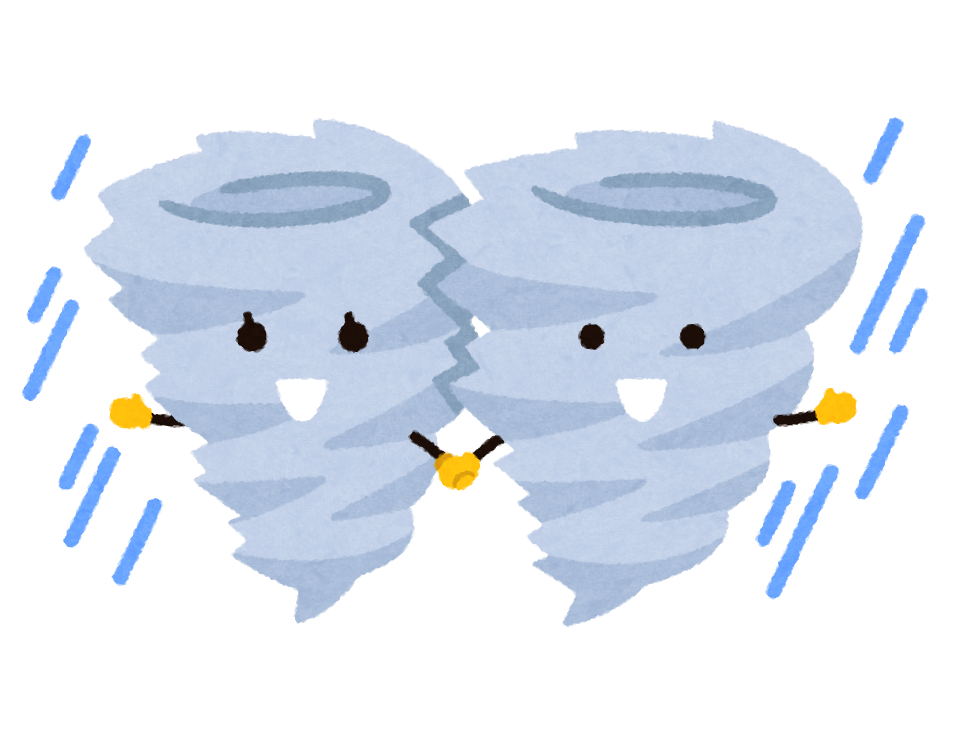
\includegraphics[width=0.5\textwidth]{sample.png}
\caption{ダブル台風のキャラクター（いらすとやより）}
\end{figure}

なお、コンパイル時に「ICCプロファイルのチェックサム不一致」という警告（Dvipdfmxによるビックリマークマークの警告）が出ることがある。
これは実害はないため無視してよい。

とはいえうざい。
ICCプロファイルを消す方法はいろいろあるが、pythonを使う方法を紹介する。
この3行だけで消せて便利である。

\begin{quote}
\begin{verbatim}
from PIL import Image
img = Image.open("sample.png")
img.save("sample.png", icc_profile=None)
\end{verbatim}
\end{quote}

\section{基本手順}

\LaTeX 文書作成の基本手順は以下の通りです。

\begin{enumerate}
  \item ソースファイル（\texttt{.tex}）をエディタで作成する
  
  まず文章の元となるファイルを作成します。この段階ではまだPDFではありません。

  \item コンパイルしてPDFを生成する
  
  pLaTeX + dvipdfmx でPDFに変換します。

  \item PDFビューアで確認する
  
  生成されたPDFを開き、レイアウトを確認します。
\end{enumerate}


% 改ページ
\clearpage


\section{表の例}

\begin{table}[ht]

\caption{簡単な表の例}
\centering

\begin{tabular}{cccc}

\toprule
項目 & 値1 & 値2 & 値3 \\
\midrule
A & 1 & 11 & 111 \\
B & 2 & 22 & 222 \\
\bottomrule

\end{tabular}

\end{table}

\end{document}